\documentclass[5pt]{article}
\usepackage{multicol,multirow}
\usepackage{graphicx} % Required for inserting images
\usepackage[margin=0.75cm]{geometry}
\usepackage{xcolor}
\usepackage{amsmath}
\usepackage{mathtools}
\usepackage{relsize}

\usepackage[english]{babel}
\newtheorem{theorem}{Theorem}

\usepackage{empheq}
\usepackage{amsfonts}

\usepackage{tkz-euclide}
\usepackage{tikz}

\definecolor{LightGray}{gray}{0.9}

\usepackage{minted}

\DeclarePairedDelimiter\abs{\lvert}{\rvert}%
\DeclarePairedDelimiter\norm{\lVert}{\rVert}%

\makeatletter
\let\oldabs\abs
\def\abs{\@ifstar{\oldabs}{\oldabs*}}

\newcommand{\tr}[3]{
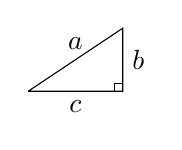
\begin{tikzpicture}[scale=0.40]
    \coordinate [] (A) at (-1.5cm,-1.cm);
    \coordinate [] (C) at (1.5cm,-1.0cm);
    \coordinate [] (B) at (1.5cm,1.0cm);
    \draw (A) -- node[above] {$a$} (B) -- node[right] {$b$} (C) -- node[below] {$c$} (A);
    \draw (1.25cm,-1.0cm) rectangle (1.5cm,-0.75cm);
\end{tikzpicture}
}


\begin{document}


\begin{center}
     \Large{\textbf{Discrete Structures}}\\
     \small{Class: APPM 1360}\hfill\small{\textcopyright Maximilien Notz \the\year{}}
     \noindent\rule{20.2cm}{0.4pt}
\end{center}


\begin{multicols}{2}
\setcounter{secnumdepth}{0}


\section{Boolean algebra}
\subsection{Boolean Identity's}
\begin{tabular}{ll}
    DeMorgan Laws    & $\lnot(a\lor b)\equiv \lnot a\land\lnot b$\\
                     & $\lnot(a\land b)\equiv \lnot a\lor\lnot b$\\
                     & $\lnot\forall x\;\beta(x)\equiv\exists x\;\lnot\beta(x) $\\
                     & $\lnot\exists x\;\beta(x)\equiv\forall x\;\lnot\beta(x) $\\
    Distributivity   & $a\land(b\lor c)\equiv(a\land b)\lor(a\land c)$\\
                     & $a\lor(b\land c)\equiv(a\lor b)\land(a\lor c)$\\
    Elimination      & $a\land T\equiv a$\\
                     & $a\land F\equiv F$\\
                     & $a\lor F\equiv a$\\
                     & $a\lor T\equiv T$\\
\end{tabular}

\section{Implications and equivalence Identity}

\section{Proof}

\section{Naive Set's Theory}
\subsection{Definitions}
\begin{tabular}{ll}
    Union             & $a\cup b=\{x\in U|x\in a\lor x\in b\}$  \\
    Intersection      & $a\cap b=\{x\in U|x\in a\land x\in b\}$ \\
    Difference        & $A-B=A\cap\overline{B}=\{x|x\in A\land x\notin B\}$\\
    Cartesian Product & $A\times B=\{(a,b)|a\in A\land b\in B\}$\\
                      & $A_1\times ...\times A_n$\\
                      & $=\{(a_1\times ...\times a_n)|a_i\in A_i$ for $i=1,...,n\}$\\
                      & $\{a,b\}\times \{0,1\}=\{(a,0),(a,1),(b,0),(b,1)\}$\\
                      
    Power Set         & The power set $\wp(E)$ is the set of all sub sets\\
                      & of $E.$\\
    Intervals         & $[a,b]=\{x|a\leq x\leq b\}$\\
                      & $(a,b)=\{x|a< x< b\}$\\
    Proper subset     & $A \subset B$\\
                      & $=\forall x(x\in A \rightarrow x\in B)\land\exists x(x\in B \land x\notin A)$\\
    Subsets           & $A \subseteq B=\forall x(x\in A \rightarrow x\in B)$\\
    A disjoint B.     & $A\cap B=\emptyset$\\
\end{tabular}
\begin{tabular}{c}
    \hline
    The sets $A$ and $B$ are equal if $A \subseteq B$ and $B \subseteq A$.\\
    \hline
    Let $S$ be a set. If there are exactly $n$ distinct elements in $S$\\ where $n$ is a non negative integer, we say that $S$ is a \textit{finite} set\\ and that $n$ is the cardinality($|S|$) of $S$.
\end{tabular}

\subsection{Identities}
\begin{tabular}{ll}
    Identity            & $A\cap U=A$ \\
                        & $A\cup \emptyset=A$ \\
    Domination laws     & $A\cup U=U$ \\
                        & $A\cap \emptyset=\emptyset$ \\
    Idempotent laws     & $A\cap A = A$ \\
                        & $A\cup A = A$ \\
    Complementation law & $\overline{(\overline{A})}=A$ \\
    Commutative law     & $A\cap B=B\cap A$\\
                        & $A\cup B=B\cup A$\\   
\end{tabular}

\section{Modular Arithmetic}
\begin{tabular}{ll}
    $a$ is divisebla by $b$ & $a|b$ \\
    $a$ congruent to $b$  & $b\equiv a(\text{mod}\; N)$\\
    $a$ congruent to $b$  & $a\equiv b(\text{mod}\; N)$\\
\end{tabular}

\section{Counting}

\section{Discrete Probability's}
\subsection{Definition}
$S$ is the a finite nonempty sample space of equally likely outcomes, and $E\subseteq S$, the the probabilitie of $E$ is $p(E)=\frac{|E|}{|S|}$.

\subsection{Some Probability Theorems}
\begin{tabular}{l}
    $p(\overline{E})=1-p(E)$\\
    $p(E_1\cup E_2)=p(E_1)+p(E_2)-p(E_1\cap E_2)$\\
\end{tabular}


\subsection{Theorems}
\begin{theorem}
For every set S, $\emptyset\subseteq S$ and $S\subseteq S$.
\end{theorem}

\begin{theorem}
Consider $f:\mathbb{Z}\rightarrow\mathbb{R}$ and $g:\mathbb{Z}\rightarrow\mathbb{R}$\\
We say $f(x)$ is $\mathcal{O}(g(x))$ if there exist constants $C$ and $k$ such that\\
$|f(x)|\le C|g(x)|$ whenever $x>k$.
\end{theorem}

\begin{theorem}[Def modulo]
    Let $m\in\mathbb{Z}^+$. $a\equiv b(\text{mod}\; m)$ if and only if $\exists k  (a=b+km)$. Where $a$ and $b$ are $\mathbb{Z}$
\end{theorem}

\begin{theorem}[Fermat little thm]
    $a^{p-1}\equiv1(\text{mod}\;p)$
\end{theorem}

\begin{theorem}
    Let $m$ be a positive integer. If $a\equiv b(\text{mod}\; m)$ and $c\equiv d(\text{mod}\;m)$, then $b+d\equiv b+d(\text{mod}\; m)$ and $bd\equiv bd(\text{mod}\; m)$.
\end{theorem}


\end{multicols}
\end{document}